% !TEX root = ../main.tex
% chktex-file 21
% chktex-file 46
\section{Graph Coarsening}%
\label{sec:coarse}

We will now see how the size of a graph $G$ can be reduced via \textit{graph coarsening}.
The resulting coarsened graph $G_c$ should ideally be structurally similar to $G$, i.e.\@ it should have a similar spectrum.
In this section we will first define the class of coarsening operators $C$ formally and give an intuition how they change the shape of a graph.
Then we will describe a randomized algorithm to compute such a coarsening.

\subsection{Definition of the Coarsening Operator}%
\label{sec:coarse:formal}

The core idea of graph coarsening is to replace clusters of vertices in the original graph $G$ by single vertices in the coarsened graph $G_c$.
Formally this means that the original vertices $\mathcal{V} = \{ v_1, \dots, v_N \}$ are mapped to a smaller vertex set $\mathcal{V}_c = \{ v'_1, \dots, v'_n \}$ via a surjective mapping $\varphi: \mathcal{V} \to \mathcal{V}_c$.
The original edges $(v_i, v_j) \in \mathcal{E}$ are mapped to $(\varphi(v_i), \varphi(v_j))$, resulting in a reduced edge set $\mathcal{E}_c$ that contains every edge for which $\varphi(v_i) \neq \varphi(v_j)$.
Figure~\ref{fig:coarse:example:coarsened} shows an exemplary graph coarsening.
To reverse the coarsening mapping, we define $\varphi^{-1}: \mathcal{V}_c \to \mathcal{P}(\mathcal{V})$ as the mapping from a coarsened vertex to the set of original vertices it represents.

\begin{figure}
	\centering
	\begin{subfigure}{0.32\textwidth}
		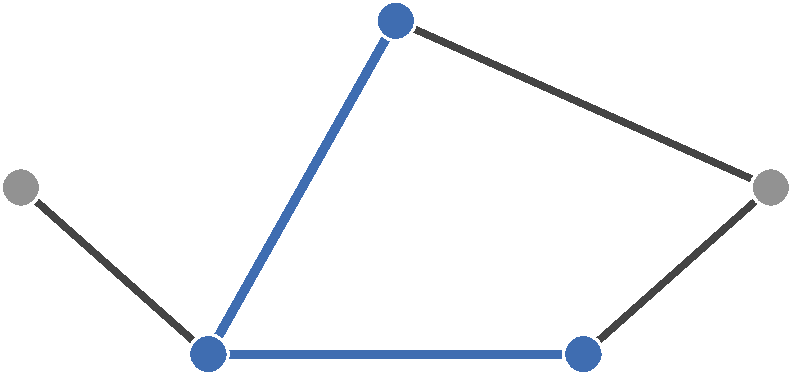
\includegraphics[width=0.9\linewidth]{gfx/coarse/example/original.pdf}
		\caption{Original $G$}\label{fig:coarse:example:original}
	\end{subfigure}
	\begin{subfigure}{0.32\textwidth}
		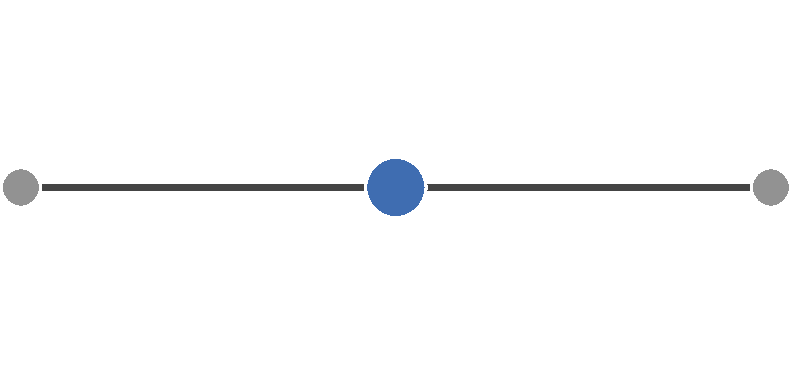
\includegraphics[width=0.9\linewidth]{gfx/coarse/example/coarsened.pdf}
		\caption{Coarsened $G_c$}\label{fig:coarse:example:coarsened}
	\end{subfigure}
	\begin{subfigure}{0.32\textwidth}
		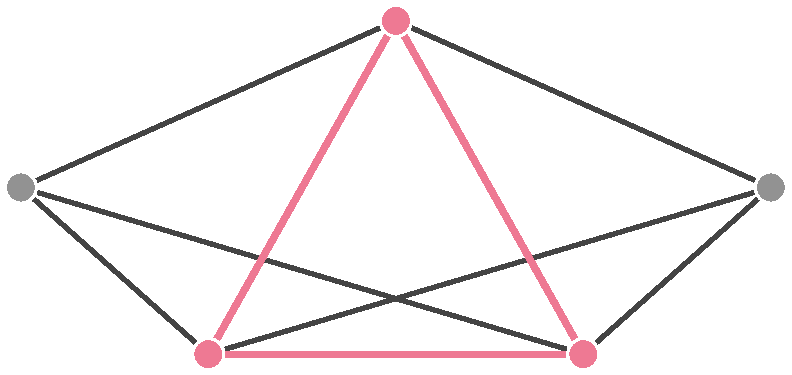
\includegraphics[width=0.9\linewidth]{gfx/coarse/example/reexpanded.pdf}
		\caption{Approximated $\widetilde{G}$}\label{fig:coarse:example:reexpanded}
	\end{subfigure}
	\caption{
		Example showing the effect of coarsening $G$ when merging the blue vertices into a single vertex.
		The graph $\widetilde{G}$ on the right shows the result of re-expanding $G_c$.
	}\label{fig:coarse:example}
\end{figure}
In the last section we saw how graphs can be described via their Laplacian $L$.
Since our goal is to analyze the effects of coarsening on the overall characteristics of a graph, we will now describe a coarsening $\varphi$ as an operation that acts directly on $L$.
The so called coarsening matrix $C \in \mathbb{R}^{n \times N}$ is essentially just a matrix representation of $\varphi$, i.e.\@ $\varphi(v_i) = v'_j \Leftrightarrow C b_i \propto b'_j$, with $b_i$ being the $i$-th standard basis vector of $\mathbb{R}^N$ and $b'_j$ the $j$-th standard basis vector of $\mathbb{R}^n$.
By linearity any signal $x \in \mathbb{R}^N$ on $G$ can thus be downsampled to a signal $x_c := C x \in \mathbb{R}^n$ on the coarsened graph $G_c$;
the signal strengths of merged vertices will simply be added up.
Similarly a downsampled signal $x_c$ can be upsampled again to an approximation $\widetilde{x} \in \mathbb{R}^N$ of the original signal $x$.
Upsampling uniformly distributes the signal strength of each $v'_j \in \mathcal{V}_c$ among $\varphi^{-1}(v'_i)$, where the inverse $\varphi^{-1}$ can be represented by $C^{\top}$:
\begin{align}
	\widetilde{x} := C^{\top} x_c = C^{\top} C x = \Pi x\quad\text{with } \Pi := C^{\top} C
\end{align}

Since both the coarsening matrix $C$ and the Laplacian $L$ are operators acting on signals, we can combine them to define the so called \textit{coarsened Laplacian} $L_c$ and the \textit{approximate Laplacian} $\widetilde{L}$:
\begin{align}
	L_c := C L C^{\top}\quad\text{and}\quad\widetilde{L} := C^{\top} L_c C = \Pi L \Pi
\end{align}
$L_c$ represents the Laplacian of the coarsened graph $G_c$\footnote{
	$L_c$ is actually not a proper combinatorial Laplacian, i.e.\@ its rows do not generally add up to $0$.
	To fix this, $L_c$ could be normalized, which is however not necessary for our analysis.
	We refer to TODO for the details.
}.
$\widetilde{L}$ represents the Laplacian of the graph $\widetilde{G}$, which is the result of re-expanding the coarsened graph $G_c$.
During re-expansion, every vertex $v'_i \in \mathcal{V}_c$ is replaced by the complete graph over the vertex set $\varphi^{-1}(v'_i)$.
The neighbors of each replaced $v'_i$ are connected to the vertices that replace it.
Figure~\ref{fig:coarse:example:reexpanded} shows how a graph might look like after such a re-expansion.

Until now we have focused on how coarsening changes the nodes and edges of a graph.


\subsection{The Randomized Edge Contraction Algorithm}%
\label{sec:coarse:rec}
